\documentclass[a4paper,12pt]{article}

\usepackage{prettylatex}
\usepackage{titlepage}
\usepackage{boiboites}
\usepackage{pgfplots}

\top{Université de Technologie de Belfort-Montbéliard}{}
\title{Cours d'IN41}{Chapitre 4 -- Numérisation des signaux}
\author{}
\date{Semestre de printemps 2016}

\newboxedtheorem[boxcolor=orange, background={rgb:white,20;green,2;black,1}, titlebackground={rgb:white,15;green,5;black,3},
titleboxcolor = black]{defi}{Définition}{cmpDefi}

\begin{document}

\maketitlepage

\tableofcontents
\pagebreak

\section{Chaine de traitement de signal}

\begin{center}
    Signal analogique \\
    $\downarrow$ \\
    Acquisition (convertisseur analogique-numérique) \\
    $\downarrow$ \\
    Traitement numérique (calculateur) \\
    $\downarrow$ \\
    Restitution (convertisseur numérique-analogique) \\
    $\downarrow$ \\
    Signal analogique
\end{center}

\section{Échantillonage}

Avant le traitement numérique par un calculateur, un signal doit être représenté par une suite de valeurs numériques prélevées régulièrement (échantillonage).

On obtient la séquence $(x_n)_{n \in \mathbb{Z}}$ avec $x_n = x(nT_e)$.

L'intervalle de temps $T_e$ séparant deux mesures successives est appelé période d'échantillonnage.

\subsection{Analyse temporelle}

\[ x_e(t) = x(t) \times \dirac_{T_e}(t) \]

\subsection{Analyse fréquentielle}

\[ x_e(t) = x(t) \times \dirac_{T_e}(t) = x(t) \sum_{k = -\infty}^{+\infty} \delta(t-kT_e) \]
\[ X_e(if) = \TF{ x_e(t)} = \TF{ x(t)} \otimes \TF{ \dirac_e(t)} \]
\[ X_e(if) = X(if) \otimes \dfrac{1}{T_e} \dirac_{\frac{1}{T_e}}(f) = X(if) \otimes f_e \dirac_{f_e}(f) \]
\[ \text{car } \TF{\dirac_{T_e}(t)} = f_e \dirac_{f_e}(f) \]

Donc le spectre de base $X(if)$ est répété en tous les multiples de la fréquence d'échantillonnage $f_e$.
\[ X_e(if) = X(if) \otimes f_e \dirac_{f_e}(f) = f_e \sum_{k = -\infty}^{+\infty} X(i(f-kf_e)) \]

\begin{figure}[!htbp]
	\centering
    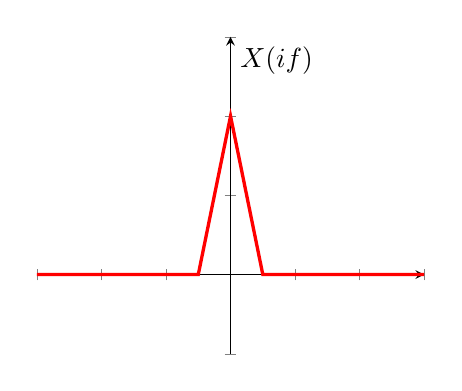
\begin{tikzpicture}
    	\begin{axis}[
            small, axis x line=middle, axis y line=center, ylabel=$X(if)$, xmin=-6, xmax=6, ymin=-0.5, ymax=1.5,
            xticklabels={,,}, % to hide the numbers on the x axis
            yticklabels={,,} % to hide the numbers on the y axis
            ]
            \addplot+[very thick, red, mark=none, sharp plot] coordinates {(-6,0) (-1,0) (0,1) (1,0) (6,0)};
    	\end{axis}
    \end{tikzpicture}
    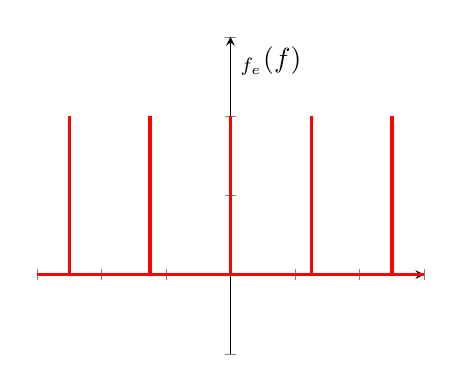
\begin{tikzpicture}
    	\begin{axis}[
            small, axis x line=middle, axis y line=center, ylabel=$\dirac_{f_e}(f)$, xmin=-6, xmax=6, ymin=-0.5, ymax=1.5,
            xticklabels={,,}, % to hide the numbers on the x axis
            yticklabels={,,} % to hide the numbers on the y axis
            ]
            \addplot+[very thick, red, mark=none, const plot] coordinates {(-6,0) (-5,1) (-5,0) (-2.5,1) (-2.5,0) (0,1) (0,0) (2.5,1) (2.5,0) (5,1) (5,0) (6,0)};
    	\end{axis}
    \end{tikzpicture}
    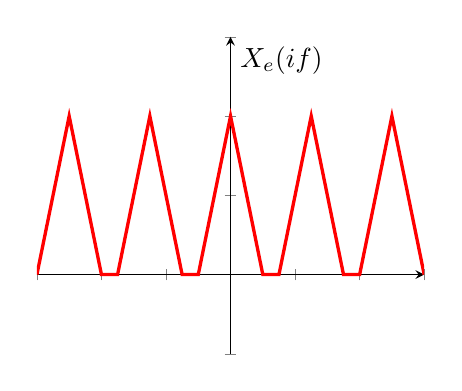
\begin{tikzpicture}
    	\begin{axis}[
            small, axis x line=middle, axis y line=center, ylabel=$X_e(if)$, xmin=-6, xmax=6, ymin=-0.5, ymax=1.5,
            xticklabels={,,}, % to hide the numbers on the x axis
            yticklabels={,,} % to hide the numbers on the y axis
            ]
            \addplot+[very thick, red, mark=none, sharp plot] coordinates {(-6,0) (-5,1) (-4,0) (-3.5,0) (-2.5,1) (-1.5,0) (-1,0) (0,1) (1,0) (1.5,0) (2.5,1) (3.5,0) (4,0) (5,1) (6,0) (6,0)};
    	\end{axis}
    \end{tikzpicture}
	\caption{Représentation de l'analyse fréquentielle}
\end{figure}

\paragraph{Principe}

Répétition du spectre de base autour de $kf_e \implies$ spectres qui vont se superposer si $f_e$ est trop petite. Si on réduit $f_e$, on diminue la distance entre les spectres qui, pour finir, se recouvrent (recouvrement spectral).

\begin{defi}[Théorème d'échantillonnage (ou de Nyquist–Shannon)]
    Un signal x(t) peut être représenté par une suite de valeurs échantillonnées si la fréquence d'échantillonnage $f_e$ est au moins deux fois plus élevée que la plus grande de fréquences contenue dans le signal.
    \[ f_e > 2f_{max} \Leftrightarrow T_e < \dfrac{T_{min}}{2} \]
\end{defi}

\subsection{Types d'échantillonnage}

\subsubsection{Échantillonnage idéal}

Échantillonnage impliquant des impulsions infiniment courtes (n'est pas réalisable physiquement).

\subsubsection{Échantillonnage réel}

La modélisation de l'échantillonnage par $\dirac_{T_e}(t)$ est erronée (impossible d'obtenir des impulsions de durée nulle). Par conséquent, chaque impulsion va avoir une durée très courte $\tau$ donc l'échantillonnage est modélisé par la multiplication de $x(t)$ par une suite d'impulsions rectangulaires de largeur $\tau$ (train d'impulsions).

\subsubsection{Échantillonnage naturel}

Amplitude égale à $x(t)$ pendant la durée $\tau$

\[ \mathrm{tr}(t) = \mathrm{rect}_\tau \otimes \underbrace{\sum_{k=-\infty}^{+\infty} \delta(t-kt_e)}_{\dirac_{T_e}(t)} \]
\[ \mathrm{TR}(f) = [\tau \mathrm{sinc}(\tau \pi f)] \times [f_e \dirac_{f_e}(f)] = \tau f_e \mathrm{sinc}(\tau \pi f) \sum_{k=-\infty}^{+\infty} \delta(f-kf_e) \]

\[ x_e(t) = x(t) \times \mathrm{tr}(t) \]
\[ X_e(if) = X(if) \otimes \mathrm{TR}(if) = X(if) \otimes [\tau f_e \mathrm{sinc}(\tau \pi f) \sum_{k=-\infty}^{+\infty} \delta(f-kf_e)] \]
\[ X_e(if) = X(if) \otimes [\tau f_e \sum_{k=-\infty}^{+\infty} \mathrm{sinc}(\tau \pi kf_e) \delta(f-kf_e)] \]
\[ X_e(if) = \tau f_e \sum_{k=-\infty}^{+\infty} \mathrm{sinc}(\tau \pi kf_e) X(f-kf_e) \]

On retrouve la même allure de spectre modulé en amplitude par un sinus cardinal ; l'échantillonnage provoque une déformation du signal.

Expression du spectre initial :
\[ X_{e_0}(f) = \tau f_e X(if) \xrightarrow{\mathrm{TF}^{}} x_{e_0}(t) = \tau f_e x(t) \]

\subsubsection{Échantillonnage régulier (ou bloqueur)}

Amplitude constante et égale à $x(kT_e)$ pendant la durée $\tau$

\[ x_e(t) = \sum_{k=-\infty}^{+\infty} x(kT_e) \mathrm{rect}_{T_e}((t-kT_e)-\dfrac{T_e}{2}) = x(t) \sum_{k=-\infty}^{+\infty} \mathrm{rect}_{T_e}(t-kT_e-\dfrac{T_e}{2}) \]
\[ x_e(t) = (x(t) \dirac_{T_e}(t)) \otimes \mathrm{rect}_{T_e}(t-\dfrac{T_e}{2}) \]
\[ X_e(if) = [X(if) \otimes f_e \dirac_{f_e}(f)] \times [T_e \mathrm{sinc}(\pi T_e f) e^{-i\pi fT_e}] \]
\[ X_e(if) = \mathrm{sinc}(\pi fT_e) e^{-i\pi fT_e} \sum_{k=-\infty}^{+\infty} X(f-kf_e) \]

Expression du spectre initial :
\[ X_{e_0}(f) = e^{-i\pi fT_e} \mathrm{sinc}(\pi fT_e) X(f) \]

Le spectre $X_e(f)$ n'est pas identique au spectre $X(f)$ puisque son amplitude est modulée par la fonction sinus cardinal. L'échantillonnage régulier introduit une déformation du signal par rapport à l'échantillonnage idéal ou naturel.

\subsubsection{Échantillonnage moyenneur}

Amplitude égale à la moyenne de $x(t)$ sur l'intervalle $\tau$

\[ x_e(kT_e) = \dfrac{1}{\tau} \int_{kT_e - \frac{\tau}{2}}^{kT_e + \frac{\tau}{2}} x(t) \mathrm{d}t \]

En utilisant la fonction fenêtre rectangulaire :
\[ x_e(kT_e) = \dfrac{1}{\tau} \int_{kT_e - \frac{\tau}{2}}^{kT_e + \frac{\tau}{2}} \mathrm{rect}_\tau(t-kT_e) x(t) \mathrm{d}t \]
\[ x_e(kT_e) = \dfrac{1}{\tau} [\mathrm{rect}_\tau(t) \otimes x(t)] \delta(t-kT_e) \]
\[ x_e(t) = \dfrac{1}{\tau} \sum_{k = -\infty}^{+\infty} [\mathrm{rect}_\tau (t) \otimes x(t)] \delta(t-kT_e) \]
\[ x_e(t) = \dfrac{1}{\tau} [\mathrm{rect}_\tau (t) \otimes x(t)] \dirac_{T_e}(t) \]
\[ X_e(f) = \dfrac{1}{\tau} [\tau \mathrm{sinc}(\pi \tau f) X(f)] \otimes f_e \dirac_{f_e}(f) \]
\[ X_e(f) = f_e \sum_{k=-\infty}^{+\infty} \mathrm{sinc}(\pi \tau (f-kf_e)) X(f-kf_e) \]

Expression du spectre initial :
\[ X_{e_0}(f) = f_e \mathrm{sinc}(\pi \tau f) X(f) \]

Extraction d'un signal à partir d'un signal échantillonné (pour obtenir $x(t)$ à partir de $x_e(t)$) :
\[ X_e(f) = f_e \sum_{k=-\infty}^{+\infty} X(f-kf_e) \]

En utilisant un filtre passe-bas idéal de fréquence de coupure $f_c = \dfrac{f_e}{2}$, on peut réaliser l'extraction du signal. La fonction réalisée par le filtre est la fonction fenêtre $\mathrm{rect}_{f_e}(f)$.

\begin{defi}[Théorème de la transformée inverse de la fenêtre rectangulaire]
    \[ \mathrm{TF}^{-1} \{ \mathrm{rect}_{f_e}(f) \} = f_e \mathrm{sinc}(\pi f_e t) \]
\end{defi}

Le spectre de base s'exprimera par :
\[ X_{e_0}(f) = X_e(f) \mathrm{rect}_{f_e}(f) \]
\[ x_{e_0}(t) = x_e(t) \otimes f_e \mathrm{sinc}(\pi f_et) \]
\[ x_{e_0}(t) = x_e(t) \otimes f_e \mathrm{sinc}(\pi f_e t) \]
\[ \text{or } x_e(t) = \sum_{-\infty}^{+\infty} x(kT_e) \delta(t-kT_e) \]
\[ \implies x_{e_0}(t) = f_e (\sum_{-\infty}^{+\infty} x(kT_e) \delta(t-kT_e)) \otimes \mathrm{sinc}(\pi f_e t) \]
\[ x_{e_0}(t) = f_e \sum_{-\infty}^{+\infty} x(kT_e) \mathrm{sinc}(\pi f_e (t=kT_e)) \]
\[ \text{d'autre part } X_{e_0}(f) = f_e X(f) \]
\[ \implies \mathrm{TF}^{-1} \{ X_{e_0}(f) = f_e x(t) \} \]
\[ \implies x_{e_0}(t) = f_e x(t) \]
\[ \implies x(t) = \dfrac{1}{f_e} x_{e_0}(t) \]
\[ x(t) = \sum_{-\infty}^{+\infty} x(kT_e) \mathrm{sinc}(\pi f_e (t-kT_e)) \]

\section{Quantification des signaux}

Quantifier un signal revient à approximer sa valeur par une valeur discrète la plus proche.

\begin{defi}[Le pas de quantification]
    Le convertisseur effectue la numérisation du signal analogique et délivre des séquences codées avec un pas de quantification $Q$ dépendant du nombre de bits de convertisseur.

    \[ Q = \dfrac{\Delta_{\mathrm{CAN}}}{2^n} \]

    \[ \text{avec } \begin{cases}
        \Delta_{\mathrm{CAN}} & \text{ le domaine de conversion du convertisseur} \\
        n & \text{ le nombre de bits}
    \end{cases} \]

    Résolution d'un convertisseur :
    \[ R_\mathrm{CAN} = \dfrac{Q}{\Delta_\mathrm{CAN}} = \dfrac{1}{2^n} \]

    Erreur de quantification :
    \[ E_Q = \dfrac{Q}{2} \]
\end{defi}

\section{Codage des signaux}

Le codage consiste à attribuer à chacun des $2^n$ niveaux issus de la quantification un code binaire sur $n$ bits.

\subsection{Signe de signal constant (codage unipolaire)}

Codage binaire naturel :
\[ N = \sum_{i=0}^{n-1} b_i 2^i = b_0 2^0 + ... + 2^{n-1} b_{n-1} \]
\[ \text{avec } \begin{cases}
    b_{n-1} & \text{ le MSB (Most Significant Bit)} \\
    b_{0} & \text{ le LSB (Least Significant Bit)}
\end{cases} \]

Au code $N$ correspond la tension $Q$.

\subsection{Signe du signal variable (codage bipolaire)}

Code d'amplitude de signe : code qui reprend le code binaire naturel avec en tête un bit de signe.

\section{Transformée de Fourier Discrète (TFD)}

Le calcul de la transformée de Fourier à l'aide d'un calculateur pose des problèmes (temps de calcul, mémoire nécessaire).
\[ \TF{x(t)} = X(f) = \int_{-\infty}^{+\infty} x(t) e^{-i2\pi ft} \d{t} \]

Cela revient à calculer une infinité d'échantillons. Il faut donc discrétiser la fonction temporelle, discrétiser la fonction fréquentielle et tronquer la fonction temporelle.

En approchant l'intégrale par une somme d'aires de rectangles de durée $T_e$ et en limitant la durée d'intégration à l'intervalle $[0, (N-1)T_e]$, on obtient :
\[ X(f) \simeq T_e \sum_{n=0}^{N-1} x(nT_e) e^{-i2\pi fnT_e} \]

On obtient pour les valeurs de fréquence $f_k = \dfrac{kf_e}{n}$ :
\[ X(f) = T_e \sum_{n=0}^{N-1} x(nT_e) e^{-i2\pi \frac{kf_e}{N} nT_e} \]

\begin{defi}[Tranformée de Fourier Discrète (TFD)]
    On appelle tranformée de Fourier discrète d'une suite de $N$ termes $\{ x(0), ..., x(N-1) \}$ la suite de $N$ termes \{ X(0), ..., X(N-1) \} définie par :
    \[ X(k) = \sum_{n=0}^{N-1} x(n) e^{\frac{-i2\pi nk}{N}} \]

    Les $N$ termes $x(n)$ sont les échantillons d'un signal analogique échantillonné $x(n) = x(nT_e) = x_n$ et les $N$ termes $X(k)$ correspondent à une approximation de la transformée de Fourier de ce signa; aux $N$ points de fréquence $f_k = \dfrac{kf_e}{N}$ avec $k \in \{ 0, ..., N-1 \}$ c'est-à-dire $f \in [0, f_e]$.

    Inversion de la tranformée de Fourier discrète :
    \[ x(n) = \dfrac{1}{N} \sum_{k=0}^{N-1}X(k) e^{\frac{i2\pi nk}{N}} \]
\end{defi}

\begin{defi}[Théorème de Parseval]
    \[ \sum_{n=0}^{N-1} ||x(n)||^2 = \dfrac{1}{N} \sum_{n=0}^{N-1} ||x(k)||^2 \]
\end{defi}

\begin{defi}[Transformée de Fourier Rapide (TFR)]
    \[ \mathrm{TFD} \implies X(k) = \sum_{n=0}^{N-1} x(n) e^{\frac{-i2\pi kn}{N}} \]
    \[ \text{soit } \omega = e^{\frac{-i2\pi}{N}} \text{ donc :} \]
    \[ \begin{bmatrix}
        X(0) \\
        X(1) \\
        X(2) \\
        \vdots \\
        X(N-1)
    \end{bmatrix}
    = \begin{bmatrix}
        1 & 1 & 1 & \cdots & 1 \\
        1 & \omega & \omega^2 & \cdots & \omega^{N=-1} \\
        1 & \omega^2 & \omega^4 & \cdots & \omega^{2(N-1)} \\
        \vdots & \vdots & \vdots & \ddots & \vdots \\
        1 & \omega^{N-1} & \omega^{2(N-1)} & \cdots & \omega^{(N-1)(N-1)}
    \end{bmatrix} \begin{bmatrix}
        x(0) \\
        x(1) \\
        x(2) \\
        \vdots \\
        x(N-1)
    \end{bmatrix} \]
    Évaluer ces sommes coûte $N^2$ produits complexes et $N(N-1)$ sommes complexes.

    Pour calculer la transformée de Fourier discrète en temps réel, on dispose d'algorithmes de calcul permettant d'obtenir les résultats beaucoup plus rapidement.

    Ces algorithmes sont connus sous le nom de transformée de Fourier rapide (TFR) ou fast Fourier transform (FFT).

    Le plus connu des algorithmes FFT est celui de Cooley-Tukey qui réduit à $N \log(N)$ le nombre de multiplications complexes.
\end{defi}

\textbf{Applications :}

On comsidère la suite $x(n)$.
\[ x(n) = \begin{cases}
    1 & \text{si } n \in \{ -1, 0, 1 \} \\
    \dfrac{1}{2} & \text{si } n \in \{ -2, 2 \} \\
    0 & \text{si } n \in \{ -m, -(m-1), ..., -4, -3 \} \cup \{ 3, 4, ..., m-1, m \}
\end{cases} \]

\begin{figure}[!htbp]
	\centering
    \begin{tikzpicture}
    	\begin{axis}[
            axis x line=middle, axis y line=center, xmin=-5.5, xmax=5.5, ymin=-0.5, ymax=1.5]
            \addplot [only marks, red] table {
            0 1
            -1 1
            1 1
            -2 .5
            2 .5
            -3 0
            3 0
            -4 0
            4 0
            -5 0
            5 0
            };
    	\end{axis}
    \end{tikzpicture}
\end{figure}

\end{document}
